%This work is licensed under the Creative Commons License Attribution 4.0 International (CC-BY 4.0) 
%https://creativecommons.org/licenses/by/4.0/legalcode 
\documentclass[rgb]{standalone}
\usepackage{tkz-euclide}
\begin{document}
	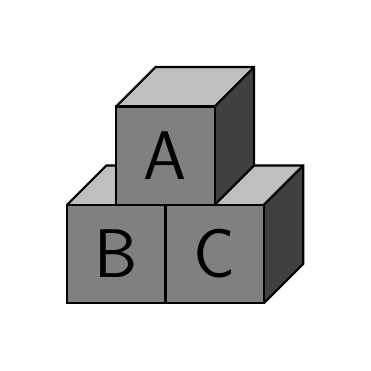
\begin{tikzpicture}[scale=0.5, font=\Large]
		\draw[draw=none] (-4,-4) -- (-4,4) -- (4,4) -- (4,-4) -- cycle;
		\draw[draw=none, fill=lightgray] (0.75,2) -- (1.75,3) -- (-0.75,3) -- (-1.75,2) -- cycle;
		\draw[draw=none, fill=lightgray] (-3,-0.5) -- (-2,0.5) -- (3,0.5) -- (2,-0.5) -- cycle;
		\draw[draw=none, fill=gray] (-3,-3) -- (2,-3) -- (2,-0.5) -- (-3,-0.5) -- cycle;
		\draw[draw=none, fill=gray] (-1.75,-0.5) -- (0.75,-0.5) -- (0.75, 2) -- (-1.75, 2) -- cycle;
		\draw[draw=none, fill=darkgray] (1.75,3) -- (1.75,0.5) -- (0.75,-0.5)  -- (0.75,2) -- cycle;
		\draw[draw=none, fill=darkgray] (2,-0.5) -- (3,0.5) -- (3,-2) -- (2,-3) -- cycle;	
		\draw[thick] (2,-3) -- (3,-2) -- (3,0.5) -- (1.75,0.5);
		\draw[thick] (-1.75,0.5) -- (-2,0.5) -- (-3,-0.5);
		\draw[thick] (0.75,2) -- (1.75,3);
		\draw[thick] (-3,-3) -- (2,-3) -- (2,-0.5) -- (-3,-0.5) -- cycle;
		\draw[thick] (-1.75,-0.5) -- (0.75,-0.5) -- (0.75, 2) -- (-1.75, 2) -- cycle;			
		\draw[thick] (-0.5,-3) -- (-0.5,-0.5);
		\draw[thick] (-1.75, 2) -- (-0.75,3) -- (1.75,3) -- (1.75,0.5) -- (0.75,-0.5);
		\draw[thick] (2,-0.5) -- (3,0.5) ;
		\tkzLabelPoint[anchor=center](-0.5,0.75){\Huge\textsf{A}}
		\tkzLabelPoint[anchor=center](-1.75,-1.75){\Huge\textsf{B}}
		\tkzLabelPoint[anchor=center](0.75,-1.75){\Huge\textsf{C}}
	\end{tikzpicture}
\end{document}